\documentclass{article} 
\usepackage{amsmath} 
\usepackage{geometry}
\usepackage{fancyhdr} 
\usepackage{graphicx} %插入图片 
\usepackage{float} %图片浮动
\usepackage{lipsum}
\usepackage{xeCJK} %调用 xeCJK 宏包 
\usepackage{array}
\usepackage{amssymb} %\mathbb 
\usepackage{ifthen} 
\usepackage{physics}
\usepackage{tikz}
\usepackage{amsthm} 
\setCJKmonofont{LXGW WenKai Mono}

\graphicspath{{./pic/}}
\geometry{left = 2.8cm, right = 2cm, top = 2cm, bottom = 3cm}
\linespread{1.48}

\begin{document}

\section*{知识点}
\subsection*{关于比值定义法}
使用比值定义法定义的物理量: 
\\
加速度$a = \dfrac{dv}{dt}$; 电场强度$E = \dfrac{F}{q}$; 电势$\varphi = \dfrac{E_p}{q}$; 磁感应强度$B = \dfrac{F}{IL}$.
\\
一些决定式: 
\\
加速度 $a = \dfrac{F}{m}$; 电场强度$E = k\dfrac{Q}{r^2}$.

\subsection*{需要注意正负的公式}
电势能$E_p = \varphi \dotproduct q$; 电场力做的功$W = q \dotproduct U_{AB}$

\subsection*{关于牛顿第二定律}
牛顿第二定律研究的是物体加速度$a$与物体质量$m$或物体所受合外力$F$之间的关系.

\subsection*{关于机械能}
除了重力之外的合力做功对应机械能的增加.

\section{题目}
\subsection{电磁}
\subsubsection*{1}
如图所示,间距$L = 1m$的U形金属导轨固定在水平绝缘桌面上,其一端接有阻值为$0.2 \Omega$的定值电阻,导轨电阻忽略不计.质量均为$m = 0.2
\text{kg}$的匀质导体棒a和b静止在导轨上,两导体棒与导轨间接触良好且始终与导轨垂直,接入电路的阻值$R_a = R_b = 0.2 \Omega $,
与导轨间动摩擦因数均为$\mu = 0.1$(设最大静摩擦力等于滑动摩擦力),导体棒a距离导轨最右端$s = 2 \text{m}$.
整个空间存在竖直向下的匀强磁场(图中未画出),磁感应强度大小$B = 0.2T$.现用沿导轨水平向右大小$F = 0.95 \text{F}$的恒力拉导体棒,
当导体棒运动到最右端时导体棒b刚要滑动.取$g = 10m/s^2$,不计空气阻力.\\
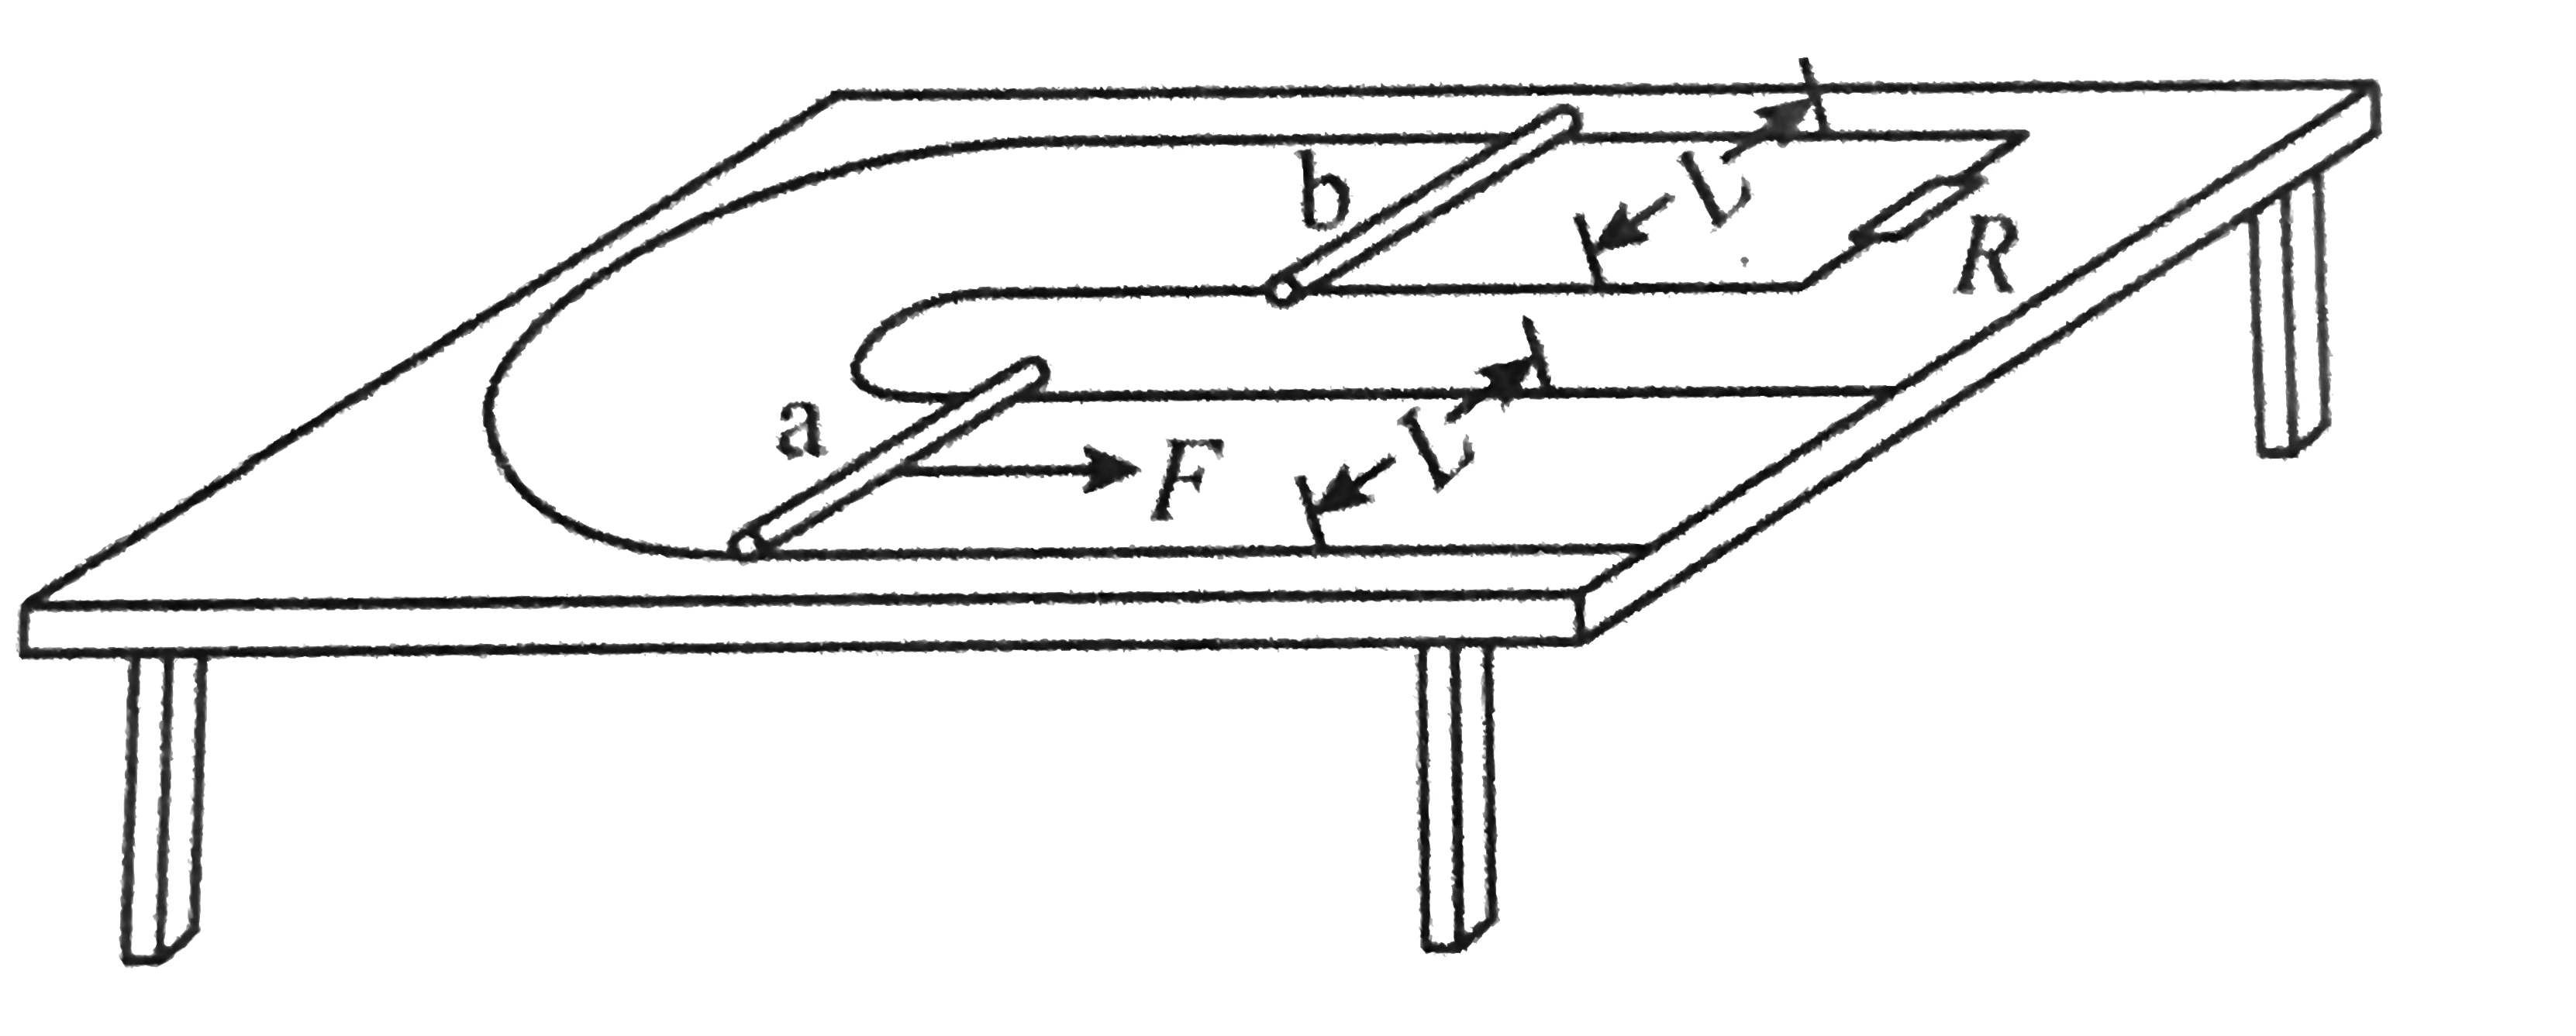
\includegraphics[height=6\baselineskip]{1.png}





\end{document}